\newcommand{\FigBentSolenoidRelativeDrift}{
\begin{figure}[t]
\centering
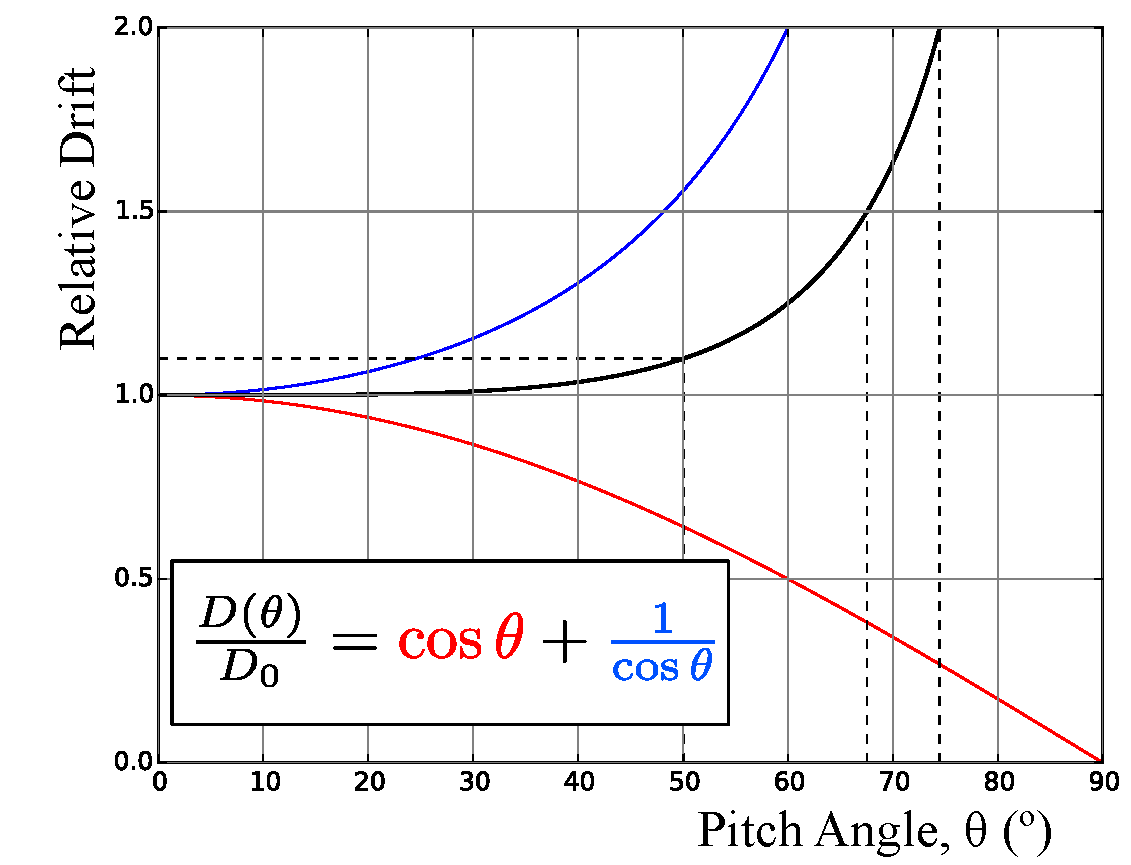
\includegraphics[width=0.6\textwidth]{figs/detector/BentSolenoids_RelativeDrift}
\caption{
Angular dependence of the magnitude of vertical drift in a bent solenoid field.
The total variation (black) remains below 10\% for pitch angles below 50\degree.
}
\figlabel{detector:bent-solenoids:angularDependence}
\end{figure}
}

\newcommand{\FigPhaseII}{
\begin{figure}[t]
\centering
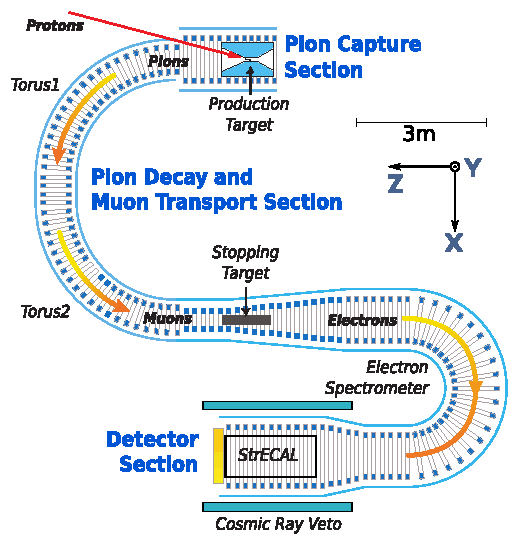
\includegraphics[width=0.9\textwidth]{figs/detector/PhaseII_schematic}
\caption{
Schematic layout of COMET \phaseII. 
The 8 GeV proton beam enters from the top-left, producing (amongst other things) pions.
Pions and muons travelling backwards with respect to the proton beam are then transported around 180 degrees of bent solenoid, during which time most of the pions decay producing an intense muon beam.
About 40\% of these muons then stop in the stopping target (centre of image).
Any electrons coming from  \mueconv are then transported through another 180 degrees of bent solenoid into the detector system.
}
\figlabel{detector:PhaseII:setup}
\end{figure}
}

\newcommand{\FigPhaseI}{
\begin{figure}[t]
\centering
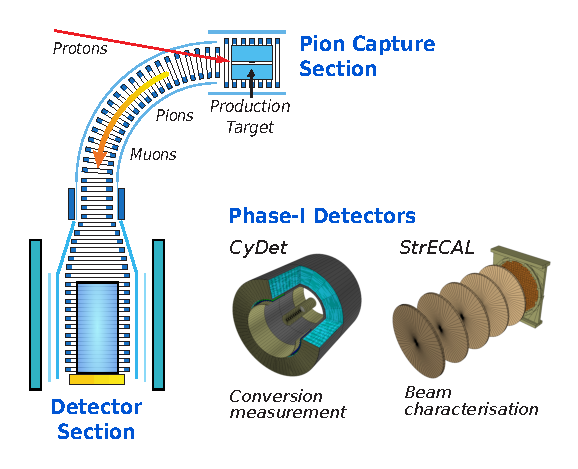
\includegraphics[height=0.4\textheight]{figs/detector/PhaseI_schematic}
\caption{
Schematic layout of COMET \phaseI. 
}
\figlabel{detector:PhaseI:setup}
\end{figure}
}

\newcommand{\TabBackgroundSummary}{
\begin{table}
\begin{tabular}{lldd}
     \hline
     \hline\\[-1.8ex]
     Type           & Background & \multicolumn{2}{c}{Predicted number of events during run} \\
                    &  & \multicolumn{1}{c}{\phaseI \cite{TDR2014}} & \multicolumn{1}{c}{\phaseII \cite{CDRphase2} } \\
     \hline\\[-1.8ex]
     Intrinsic & Muon Decay-in-Orbit                       & 0.01              & 0.15    \\
               & Radiative Muon Capture                    & 0.00056           & <0.001  \\
               & $\mu^-$ Capture w/ n Emission             & <0.001            & <0.001  \\
               & $\mu^-$ Capture w/ Charged Part. Emission & <0.001            & <0.001  \\
     Prompt    & Radiative Pion Capture                    & 0.00023           & 0.05    \\
               & Beam Electrons                            & 0.00083           & <0.1^*  \\
               & Muon Decay in Flight                      & \le0.0002         & <0.0002 \\
               & Pion Decay in Flight                      & \le0.00023        & <0.0001 \\
               & Neutron Induced                           & -                 & 0.024   \\
               & Other beam induced B.G.                   & <2.8\times10^{-6} & -       \\
     Delayed   & Delayed Radiative Pion Capture            & \sim0             & 0.002   \\
               & Anti-proton Induced                        & 0.007             & 0.007   \\
               & Other delayed B.G.                        & \sim0             & -       \\
     Cosmic    & Cosmic Ray Muons                          & -                 & 0.002   \\
               & Electrons from Cosmic Ray Muons           & <0.0001           & 0.002   \\
     \hline\\[-1.8ex]
     \multicolumn{2}{c}{Total background}                      & 0.019         & 0.34    \\
     \multicolumn{2}{c}{Signal (Assuming $B=1\times10^{-16}$)} & 0.31          & 3.8     \\
     \hline
     \hline
\end{tabular}
\caption{
	\CHECK{UPDATE \phaseI values with TDR 2016}
	Backgrounds for COMET \phaseI \cite{TDR2014} and \phaseII \cite{CDRphase2}.
	Prompt backgrounds arise by protons that occur in between bunches and are therefore suppressed by the extinction factor.
	For \phaseI, the recently measured value of $10^{-12}$ was used for the extinction factor, but for \phaseII the older expectation of $10^{-9}$ was used.
}
\tablabel{detector:backgrounds}
\end{table}
}

\newcommand{\FigMuonNuclearParams}{
\begin{figure}[bp]
\centering
\subfloat[][\figlabel{detector:mu-nucl-params:lifetimes}Lifetimes]{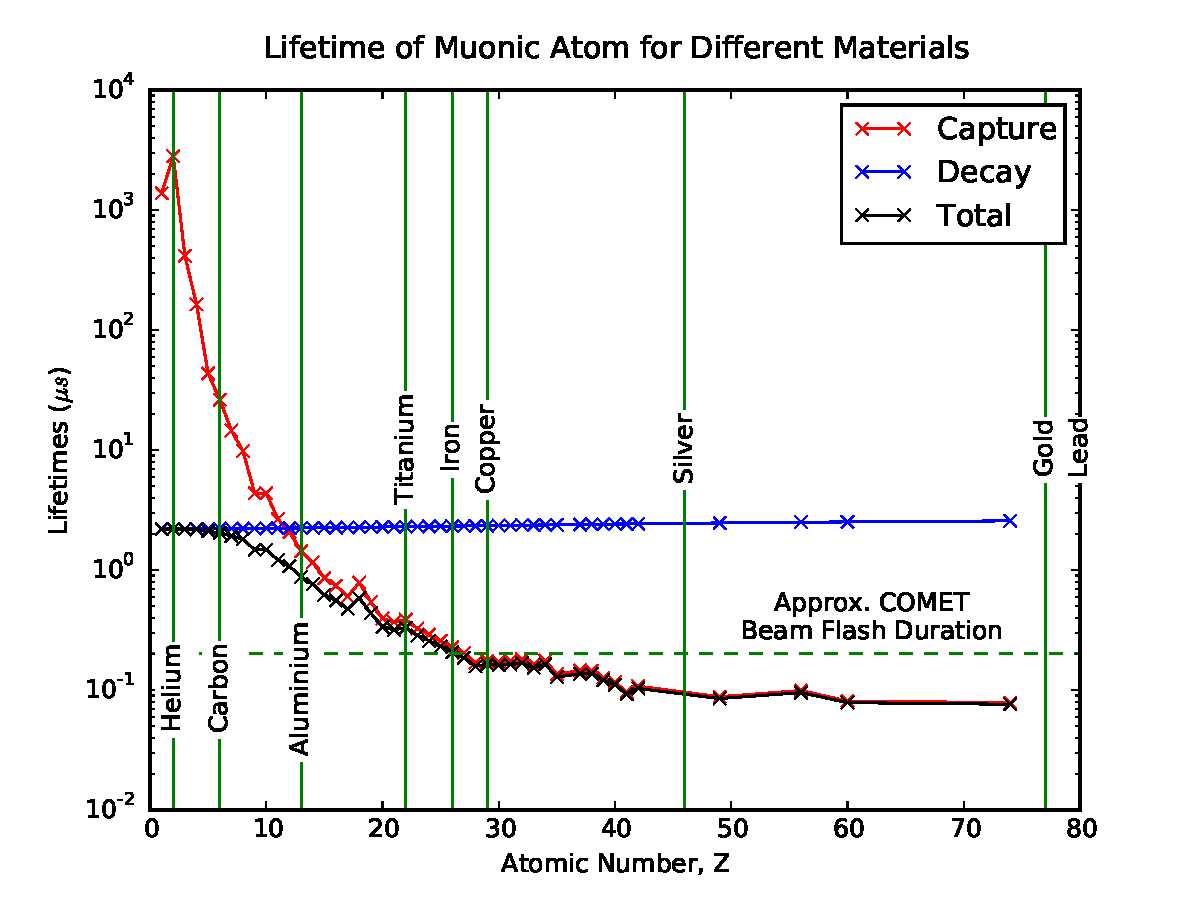
\includegraphics[width=0.9\textwidth]{figs/detector/MuNuclearParams_All_lifetimes.pdf}}\\
\subfloat[][\figlabel{detector:mu-nucl-params:end-point}End-point Shift]{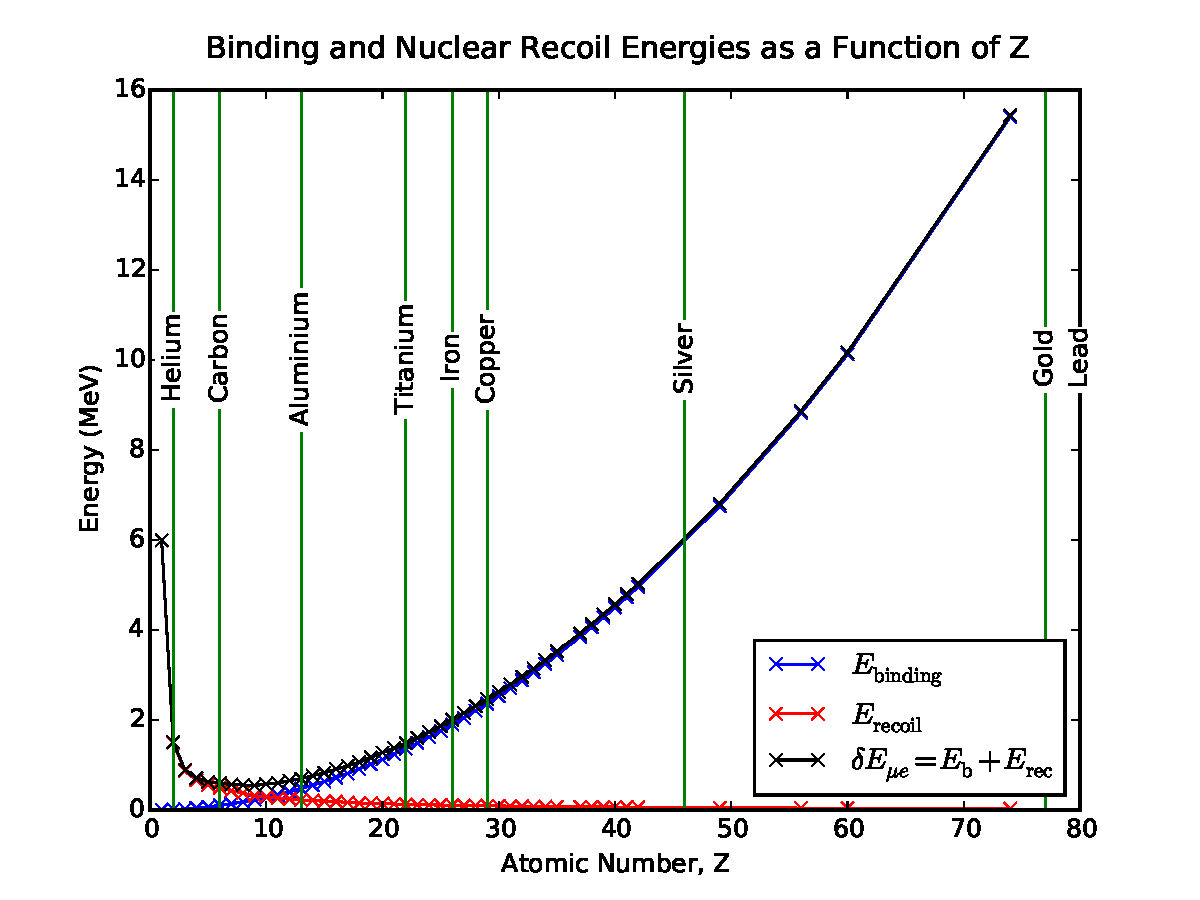
\includegraphics[width=0.49\textwidth]{figs/detector/MuNuclearParams_energies.pdf}}%\hspace{0.5cm}%
\subfloat[][\figlabel{detector:mu-nucl-params:branching-ratio}Branching Fraction]{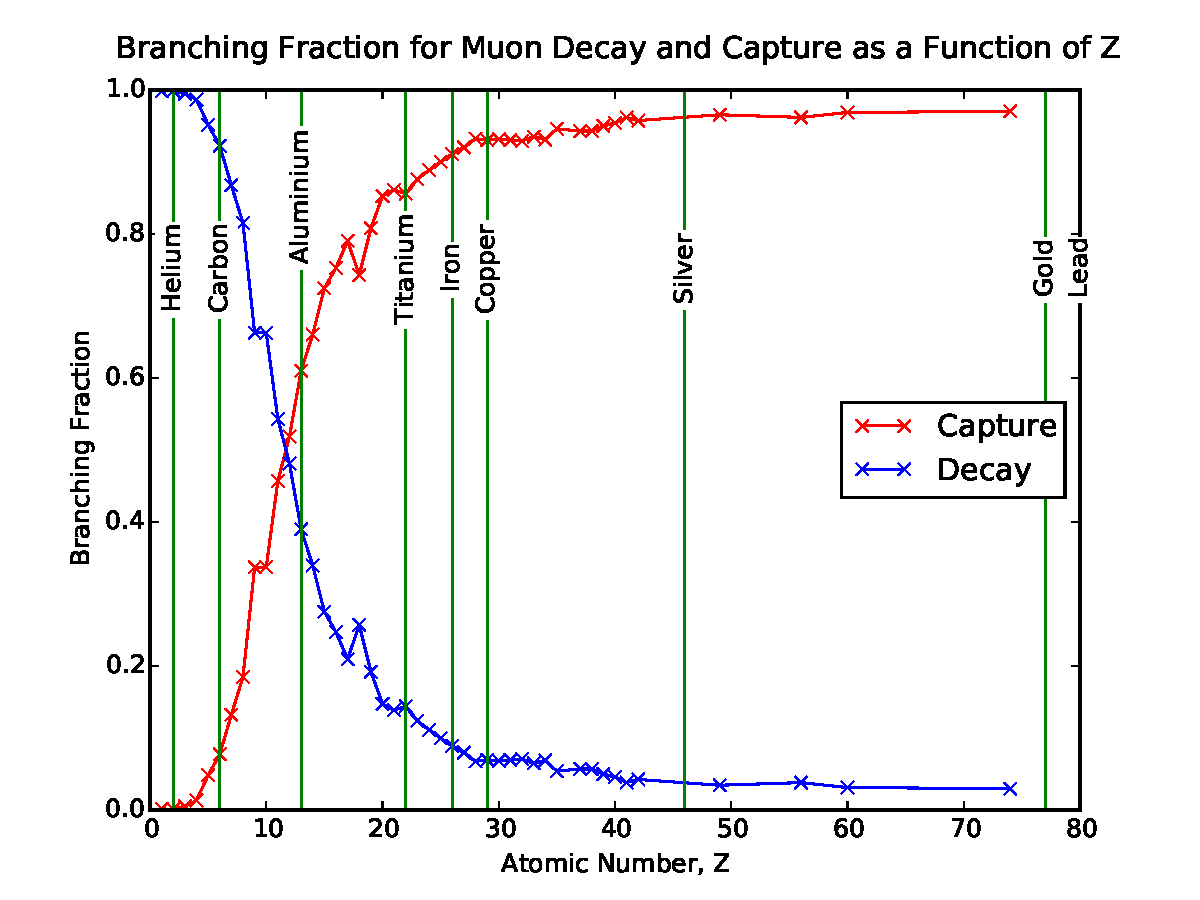
\includegraphics[width=0.49\textwidth]{figs/detector/MuNuclearParams_branching_fraction.pdf}}
\caption{\figlabel{detector:mu-nucl-params}
The effect of changing the atomic number on the branching ratio, lifetime and electron energy spectrum end-point.
For the branching ratio and lifetime plots, the partial rate for muon nuclear capture and decay-in-orbit are shown separately.
The capture and decay rates are taken from the Geant4 \cite{Geant42003} parametrisation for stopped negative muons.  
Only elements for which at least 1 isotope uses a measured value are plotted.
The values for the end-point energy level are calculated using the Bohr model for the muon ground-state binding energy.
}
\end{figure}
}


\chapter{The COMET Experiment}
%\section{Muon to Electron Conversion: Signal and Backgrounds}
% - COMET stands for COherent Muon to Electron Transitions
% - Cite the experimenter's guide by Bob Bernstein

%Introduction:
The aim of the COMET experiment is to search for COherent Muon to Electron Transitions with a single-event-sensitivity of around \sensePII.
This amounts to an improvement of four orders of magnitude compared to the current limit \cite{sindrum2006} which requires some significant changes to the way the experiment operates.

The general experimental goals of COMET are to:
\begin{itemize}
\item stop many muons in aluminium,
\item have a high signal acceptance,
\item suppress potential background sources to well below a single event.
\end{itemize}

At the level of sensitivity desired for COMET these requirements translate to the need for:
\begin{itemize}
\item a very high intensity muon beam,
\item a thin stopping target and low material budget detector,
\item a low energy muon beam,
\item a pulse beam and relatively low-Z stopping target.
\end{itemize}

Realising these goals requires many new experimental techniques and as such COMET has decided to operate in two stages, \phaseI and \phaseII.
\phaseII will realise the final objective of \sensePII, whilst \phaseI aims for a measurement with sensitivity of \sensePI but also to understand the beam and backgrounds to improve our understanding of \phaseII.
In order to understand both phases a simple appreciation of the types of backgrounds that must be considered is valuable, so I shall first give an overview of these.
%Firstly however I will discuss some of the key aspects common to both \phaseI and \phaseII.
%Although \phaseI will run sooner, since it is heavily motivated by \phaseII, I shall describe \phaseII in more depth first and return \phaseI subsequently.

\section{Overview of Signal and Backgrounds}
\TabBackgroundSummary
\mueconv is experimentally attractive because its signal is so simple: a single monoenergetic electron at close to the muon mass of 105~MeV/c, given by:
\begin{equation}
E_e=M_\mu-E_{\mu,\mathrm{binding}}-E_\mathrm{recoil}
\end{equation}
where $M_\mu=$105.66~MeV/c$^2$ is the muon mass, $E_{\mu,\mathrm{binding}}$ the
binding energy of the muon in the ground state of the muonic atom, and
$E_\mathrm{recoil}$ is the kinetic energy of the recoiling nucleus.
In the aluminium target used for COMET (see section \ref{sec:stop-tgt}) the electron energy is $E_e=104.97$~MeV.

Background rates must be kept well below the signal sensitivity if an observation is to be confidently identified as signal, or if meaningful limits are to be set.
Given the desired sensitivity of COMET is \sensePI  at \phaseI and \sensePII by \phaseII, background rates must be kept equally rare.

\Tab{detector:backgrounds} summarizes the results of previous studies for background rates at \phaseI and \phaseII.
There are predominantly four main groups of background sources: intrinsic, prompt, delayed and cosmic sources.

Intrinsic processes are those that arise from muons stopping in the target and will therefore always be present regardless of how well you make your muon beam and detector.
Of these, the dominant background is muon decay in orbit, which is the standard model process of a muon decaying to an electron, emitting two neutrinos in the process.
Although the decay of a free muon cannot produce electrons with energy greater than half the muon mass, once bound to a nucleus the neutrinos can be configured to carry almost no kinetic energy away, such that only the nucleus and electron are important in the end-point configuration.
It can immediately be seen then the kinematics of the end-point configuration for muon decay-in-orbit are the same as for \mueconv, and indeed
a tail in the spectrum of electrons coming from muon decay-in-orbit extends all the way up to this point.
\Fig{detector:DIOSpectrum} shows the spectrum of electrons from muon decay-in-orbit in aluminium where it can be seen that the high energy tail does reach up to about 105~MeV/c, but with a very steeply falling rate.

\CHECK{Figure for DIO spectrum on log / lin scales from 2011 paper, or 2015 paper?}

%Since the nucleus is so massive compared to the electron, it requires very little energy to have it conserve momentum with the out-going electron.

Delayed and prompt processes can come from impurities in the muon beam, the key difference being the timing with respect to the proton beam arrival.
For example, pions reaching the stopping target region are dangerous since they can produce high energy gamma rays which can pair produce to create 105~MeV electrons.
Since pion capture against a nucleus is extremely fast ( less than 1~ns ) the timing of pion-induced backgrounds is determined solely by the arrival time of pions into the target region.
In order to reach this region without decaying, the pions must be relatively high momentum of about 60~MeV/c or greater.  
As a result, backgrounds from pion capture are typically expected close to the arrival of protons at the production target.
These sort of prompt processes are suppressed by using a pulse proton beam (discussed in more depth later) and ensuring very few protons in between pulses.
Should a pion in the beam arrive at the target region with a large delay then the timing of the proton beam is not a useful method for suppressing this.  
Possible causes of this against which must be mitigated is the mirroring of particles in the magnetic field or by production of pions and high-energy electrons from antiprotons.
At a given momentum, antiprotons travel considerably more slowly than muons or pions given their considerably larger mass.
Other beam related issues include the decay of muons and pions to electrons.
An electron of 100 MeV/c can be produced by muons or pions with greater than 70 or 50~MeV/c respectively, and so the flux of higher energy particles must be removed.

Finally cosmic backgrounds arise from high energy muons that pass through the building and enter the detector or beamline.  
Events where a muon decays to an electron which is then detected as 105~MeV are counted as backgrounds.
In particular, muons that produce high energy electrons close to the target are dangerous since cuts on the reconstructed direction and position will be less effective.

\section{General Experimental Techniques}
\subsection{Proton Beam Energy and Production Target}
The muon beam used in COMET is produced as the decay products of a secondary pion beam created by protons striking a target.
If maximising the muon intensity were the only concern, then both the proton beam energy and atomic mass of the target material would also be maximised since the pion production cross section
grows with these two parameters.
However, the need to suppress background rates and maintain the mechanical and operational stability of the target constrain both of these parameters.

In particular, protons with more than 5.6~GeV \CHECK{Target dependence? Correct?} striking a stationary target have sufficient energy to produce antiprotons which travel relatively slowly (see \ref{sec:stop-tgt}) and can produce backgrounds.
Since the antiproton yield grows very quickly above this threshold, it has been chosen to use protons with 8~GeV kinetic energy.

For \phaseII running, the main ring will operate at 7~$\mu$A so that a beam power of 56~kW is achieved.  
\phaseI on the other hand will use a lower beam intensity of 0.4~$\mu$A or 3.2~kW.

A heavy metal target is preferable since it improves the pion yield, in particular tungsten since it is relatively cheap compared to other options.
However, at the beam powers under consideration, a metal target would melt, such that we must actively cool the target.
Such will be the approach in \phaseII, however for simplicity \phaseI will run with a radiatively cooled graphite target.

\CHECK{Figure for pion vs. antiproton production cross-section for different proton energies and/or target materials}

Finally, only those pions and muons emitted in the backwards direction with respect to the proton beam are captured and transported to the muon beamline.
This is a strong way to reduce the high-energy components of the muons and pions distributions since the yield for low momentum pions in the forward and backwards direction is similar, whilst the high energy tail is greatly suppressed in the backwards direction.
At this time however, there is a dearth of experimental measurements for pion production in the backwards direction with 8~GeV protons on a graphite or tungsten target.
\Fig{detector:piYield} shows a measurement of the cross section for pion production with 10~GeV protons on tantalum (which is adjacent to tungsten on the periodic table).

\subsection{Particle Transport through Bent Solenoids}
\FigBentSolenoidRelativeDrift
Both \phaseI and II make use of bent solenoids to help select particles of a particular momentum.
In bent solenoids, a dispersion occurs that is proportional to the momentum and charge of the particle passing through it.

Charged particles moving through a straight solenoid follow a helical
trajectory, orbiting a point that moves parallel to the solenoidal axis with constant velocity fixed by the longitudinal momentum of the particle.
The frequency that the particle rotates about this point (betatron frequency or frequency of gyration) is determined by the transverse momentum.

By comparison, if a charged particle moves through a solenoid channel that has been bent, the particle can still be considered to orbit a point, only now 
the motion of that point can be shown to drift vertically, out of the plane of bending.  This drift arises from the gradient introduced to the field by bending the solenoid but also from the 
non-rectilinear coordinate system of the field lines.  
The total drift, $D$, of a particle with mass and charge $m$ and $q$ respectively  through a solenoid bent with a fixed radius of curvature, $R$, is given by:
\begin{align}
	D=&\frac{1}{qB}\left(\frac{s}{R}\right)\frac{p^2_\mathrm{L}+0.5p^2_\mathrm{T}}{p_\mathrm{L}}\eqlabel{detector:bent-solenoids:longVstrans}\\
	 =&\frac{1}{qB}\left(\frac{s}{R}\right)\frac{p}{2}\left(\cos\theta + \frac{1}{\cos\theta}\right)\eqlabel{detector:bent-solenoids:pitchAngle}
\end{align}
where $B$ is the magnetic field strength\footnote{Strictly speaking, $B$ is the field strength along the path of the centre of gyration, which is constant for a fixed transverse distance from the focus of the bent solenoid.},
$s$ is the distance travelled through the solenoid, $p$ the momentum of the particle, with longitudinal and transverse components with respect to the solenoid axis, $p_\mathrm{L}$ and $p_\mathrm{T}$ respectively.
The pitch angle, $\theta$, is a property of the helical trajectory taken by the particle and defined as:
\begin{equation}
\theta=\tan^{-1}\left(\frac{p_\mathrm{T}}{p_\mathrm{L}}\right)
\end{equation}
See Appendix \ref{sec:appendix:bent-solenoid} for a derivation of equations \eq{detector:bent-solenoids:longVstrans} and \eq{detector:bent-solenoids:pitchAngle}.
The angular dependence of this equation is shown in \fig{detector:bent-solenoids:angularDependence} where it can be seen that for angles below 50 degrees the variation in the drift is less than 10\%, such that the drift is determined almost completely by the momentum of particles up to these angles.

Bent solenoids are used to disperse high-energy muons and pions in the muon
beam for both \phaseI and II, and as a spectrometer system for electrons coming
from the stopping target in \phaseII, which will both be described in more
detail below.

%The dynamics of a charged particle in a magnetic field is determined by the Lorentz equation:
%\begin{equation}
%\vec{F}=\frac{q}{m}\vec{p}\times\vec{B}
%\end{equation}
%where $q$, $\vec{p}$ and $m$ are the particle's charge, momentum and mass respectively, and $\vec{B}$ is the magnetic field.
%In a uniform magnetic field where all field lines are parallel, clearly the motion of the particle follows a helix whose axis is parallel to the field and
%with a helical pitch-angle given by:
%\begin{equation}
%\theta=\tan^{-1}\Big(\frac{P_\mathrm{T}}{P_\mathrm{L}}\Big)
%\end{equation}
%where $P_\mathrm{T}$ and $P_\mathrm{L}$ are respectively the transverse and longitudinal components of the momentum with respect to the magnetic field.
%Such a field can be realised to a high precision by a cylindrical solenoid coil.
%
%If instead one were to bend a solenoid coil, so that it's axis describes a circular arc, two effects are introduced:  firstly, the uniformity of the field is changed
%such that a higher magnetic field is found on the inside of the bend, and secondly the field lines also bend.
%Each of these changes causes the motion of the particle to deviate from that of a straight solenoid.
%Whilst one can think of the particle as following a helix around the field lines still, the centre of this helix can be shown to drift out of the plane of the bending.
%Firstly, the radial gradient introduced to the field causes a drift which is proportional to the transverse momentum of the particle.
%Secondly, the centrifugal pseudo-force as the particle tracks the now cylindrical field lines, creates a force that acts perpendicularly to the magnetic field.
%Since the field lines follow the solenoidal axis, this also produces a vertical drift, proportional to the longitudinal momentum, however.
%
%Taken together, the result is a vertical drift with a velocity given by:
%\begin{equation}
%\end{equation}

\subsection{Stopping Target Material and Beam Pulsing}
\label{sec:stop-tgt}
\FigMuonNuclearParams

The combination of using backwards going pions and the long, bent-solenoid transport channel is already effective at removing potential background issues.
In addition to these however, there is one further method which helps both to reduce beam-related backgrounds and improve the detector occupancy and reconstruction requirements:
the use of a pulsed proton beam with a relatively light stopping target.

Since the signal process is coherent, its cross section grows roughly as the square of the number of nucleons (or protons, depending on the model)%
\footnote{Although this growth is offset by the normalisation to the capture rate which is incoherent and grows linearly with the number of nucleons, so that the conversion rate itself is roughly linear.}
until the muon is contained almost completely within the nucleus at which point the rate levels off.
It is therefore desirable to use a high-Z target in order to increase the probability of conversion and indeed \sindrumII used both lead and gold targets, with its most stringent limit coming on gold \cite{sindrum2006}.

However, as the nucleus gets larger, the lifetime of the muonic atom falls steeply due to the increase in the nuclear capture rate.
This is illustrated in \fig{detector:mu-nucl-params} where it can be seen that for elements heavier than iron ($Z>26$)the muon lifetime is less than 200~ns.
The COMET beamline produces a beam flash that lasts for about 200~ns after the arrival of a proton at the production target.
This means that for targets heavier than iron timing information can not be used to distinguish particles coming from the beam or from the decay of a muon stopped in the target.

Whilst these are the two dominant factors in deciding the target material, other factors like the mechanical stability, cost, isotopic purity and the stability of the daughter nuclei following muon capture on the target must also be considered.
Accordingly, titanium and aluminium are considered the two most viable target materials.  
Titanium, in which the muon lifetime is about 330~ns, would be considerably harder to measure \mueconv so at this stage the COMET experiment is focussed on using aluminium where the muon lifetime is about 864~ns \cite{Suzuki1987}.

The J-PARC accelerator has buckets separated by 550~ns, although separations of multiples of this number can in principle be achieved.
For COMET running the intention is to fill every other bucket so that a separation of 1.17~$\mu$s is achieved.
\Fig{detector:timing-schema} shows the beam timing schematically.  
A window from about 700 to 1100~ns after the proton beam arrival is then used to look for signal events, by which time most of the beam flash should have passed whilst signal events remain probable.

Having a well-defined bunch structure is crucial for this scheme to work. 
Protons arriving in between bunches would produce (a fragment of) beam flash that could include high energy muons or pions which could result in background electrons arriving within the timing window.
The extinction factor quantifies the chance of this and is given by:
\begin{equation}
	R_\mathrm{Extinction}=\frac{N(p~\mathrm{between~bunches})}{N(p~\mathrm{per~bunch})}
\end{equation}
Original estimates were made assuming $R_\mathrm{Extinction}$ was around $10^{-9}$ \cite{CDRphase2} (about 1 out-of-time proton for every 7 bunches) although recent measurements have been able to demonstrate extinction at a level of $10^{-12}$ \cite{COMETExtinctionNote} (about 1 out-of-time proton for every 7100 bunches).

The bunch structure is initially defined by the linac at J-PARC which accelerates protons up to 600~MeV.
The \ac{RCS} then takes these protons up to 3~GeV where up to two buckets can be stored at a time, although for COMET only one bunch at a time will be filled.
The protons are then injected into the \ac{MR} which accelerates them up the final energy of 8~GeV and is capable of storing up to 9 buckets at once.
Using the Linac chopper along would not be sufficient to keep the extinction factor since stray protons tend to drift into the unfilled buckets.
Achieving the high extinction factor then is possible only by using the injection kicker from the \ac{RCS} to the \ac{MR} in a `double-kick' mode.
The kicker excitation length is set to two buckets (so that the \ac{RCS} is completely emptied into the \ac{MR}).  
The kicker is then activated again immediately after the first filled bunch has performed a complete rotation of the \ac{MR} such that protons that had diffused into the second bunch of the \ac{RCS} are now kicked away.
Thus only four out of the nine buckets in the \ac{MR} are filled and all other buckets are kept empty.

\section{\COMET \phaseI}
\FigPhaseI
% - Measurement goals
% - StrECAL detector
% - CyDet detector

There are two key goals to \phaseI:
\begin{enumerate}
\item measure \mueconv at a sensitivity of \sensePI,
\item prepare for \phaseII by measuring the beam profile, particle yields and background rates, and prototype the detector technology.
\end{enumerate}

\phaseI will see the construction of the \COMET hall, the production target capture solenoids, the first 90 degrees of the bent muon transport solenoid, and the detector solenoid.  
The beamline is shown schematically in \fig{detector:PhaseI:setup} where the two interchangeable detector systems can also be seen.

Since the dynamics of bent solenoids are complicated, it is important to study the beam as close to the production target as possible.
However, due to the high radiation environment, it is important that the detector and electronics be kept well shielded.
\phaseI will therefore measure the beam after the first 90 degrees of bent solenoid using the same detector system to be used in \phaseII, namely the \ac{StrECAL} detector -- a series of Straw Tracker stations  followed by an ECAL
all sitting in the beam.  

Since the StrECAL detector will be hit by the full force of the muon beam, it would not be feasible to conduct a \mueconv search using this detector.
As such, for \phaseI a second detector, known as the \ac{CyDet} will be used to conduct the \mueconv search.


\section{\COMET \phaseII}
COMET \phaseII will be the final stage of the experiment.
It will make use of all the above techniques

\FigPhaseII
% - Proton beam energy
% - Proton beam timing
% - Production target and capture system
% - Bent Transport system
% - Stopping target
% - Detector system

\section{Status and Schedule}
